\part{Viola-Jones algoritam}\label{viola_jones_algorithm}

\section{Uvod} \label{viola_jones_introduction}

Viola-Jones algoritam za detekciju i lokalizaciju objekata na slici razvijen je od
strane Paul Viola i Michael Jones 2001. godine \cite{Viola2001RapidOD}.\\
Zbog brze i pouzdane detekcije jedan je od nakorišćenijih algoritama za
detekciju lica na slici.
Iako danas neuronske mreže polako zamenjuju tradicionalne algoritme za detekciju
objekata, Viola-Jones algoritam je i danas prisutan u velikom broju mobilnih
telefona i digitalnih kamera. \\

Pouzdanost i brzina su postignuti uvođenjem tri ključna doprinosa:
\begin{itemize}
\item \textbf{Integralna slika} omogućava brzo izračunavanje obeležja.
\item \textbf{\gls{adaboost}} je algoritam za mašinsko učenje, odabiranjem
  obeležja povećava se brzina i pouzdanost detekcije.
\item \textbf{Kaskadni klasifikator}, organizovanjem obeležja u kaskade
  omogućava brzo odbacivanje regiona sa malom verovatnoćom pojave traženog
  objekta, npr. pozadine slike. \\
\end{itemize}


\subsection{Integralna slika} \label{ii_sec}

Kao jedan od ključnih delova algoritma, integralna slika je uveliko zaslužna za
brzinu detekcije.
Integralna slika predstavlja transformaciju originalne slike, takvu da se zbir
proizvoljnog broja piksela originalne slike može izračunati u konstantnom
vremenu.\\

Vrednost piksela integralne slike na poziciji (x, y) je zbir svih piksela koji
se nalaze u pravougaoniku gore i levo od pozicije (x, y).

\begin{equation}
  \Scale[1.4]{ii(x,y)=\sum\limits_{x'\leq x, y'\leq y} i(x',y')}
  \label{IntegralImage_eq1}
\end{equation}

Gde je ii(x,y) integralna slika, a i(x,y) originalna slika. \\

\begin{figure}[H]
  \centering
  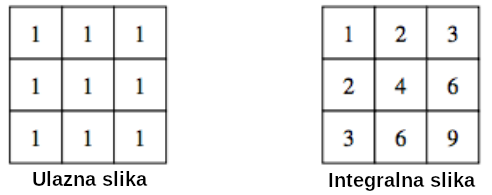
\includegraphics[width=0.55\linewidth]{integral_image1}
  \caption{Primer integralne slike}
  \label{IntegralImage_img1}
\end{figure}

Kako je u Viola-Jones algoritmu potrebno izračunavanje površine nad pravougaonim
obeležjem originalne slike.
Integralna slika donosi veliko ubrzanje prilikom ove operacije. \\
U integralnoj slici za proizvoljno pravougaono obeležje moguće je izračunati
površinu sa samo 2 oduizamanja i jednim sabiranjem. \\

\begin{figure}[H]
  \centering
  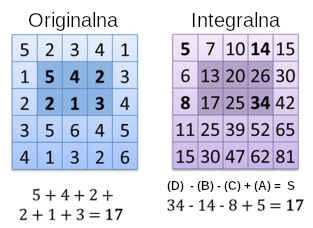
\includegraphics[width=0.55\linewidth]{integral_image2}
  \caption{Primer računanja površine pravougaonika \cite{IntegralImage1_web}}
  \label{IntegralImage_img2}
\end{figure}

Na slici (\ref{IntegralImage_img2}) je prikazano računanje površine pravougaonika na
originalnoj slici i iste površine na integralnoj slici.
Kao što se može videti za površinu pravougaonika MxN na originalnoj slici nam je
potrebno MxN-1 sabiranja. \\
Dok je kod integralne slike broj operacija 2 oduzimanja i 1 sabiranje i ne
zavisi od dimenzija pravougaonika. \\

Formula za računanje površine pravougaonika originalne slike pomoću integralne
slike prikazan je u nastavku. \\

\begin{equation}
  \Scale[1.4]{\sum\limits_{(x,y)\in ABCD} i(x,y)=ii(D)+ii(A)-ii(B)-ii(C)}
  \cite{Cen2016StudyOV}
  \label{IntegralImage_eq2}
\end{equation}

Treba napomenuti da je za transformaciju slike u integralnu potrebno značajno
računsko vreme.
Zbog toga je korišćenje integralne slike isplativo jedino ukoliko je potreban
veliki broj operacija računanja površine pravougaonika na željenoj slici, što je
slučaj u Viola-Jones algoritmu. \\

Integralnu sliku je moguće računati u paraleli ili
sekvencijalno. Izbor algoritma za računanje integralne slike značajno utiče na
performanse i potrebne hardverske resurse konačne implementacije. \\
U paralelnoj implementaciji cena je više pristupa memoriji i više potrebnih sabirača, dok je kod sekvencijalne
implementacije manja brzina proračunavanja. \\

\subsection{AdaBoost i HAAR obeležja}

\subsubsection{HAAR obeležja} \label{haar_features_sec}

Viola-Jones modeli za detekciju objekata se sastoje od mnogobrojnih HAAR obeležja.
HAAR obeležja se sastoje od dva ili više pravougaonika.
Ovi pravougaonici mogu imati svoje dimenzije i težinu.
Na slici(\ref{haar_features_img1}) prikazani su neki mogući tipovi HAAR
obeležja, crni i beli pravougaonici imaju različite težine.

\begin{figure}[H]
  \centering
  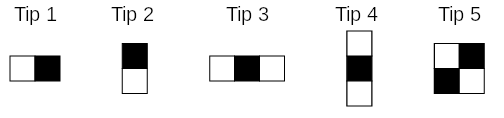
\includegraphics[width=0.55\linewidth]{haar_features1}
  \caption{HAAR obeležja \cite{Jensen2008ImplementingTV}}
  \label{haar_features_img1}
\end{figure}

HAAR obeležja imaju dimenzije manje od dimenzije slike, tipične dimenzije ovih
obeležja su oko 24x24 piksela. \\
Prilikom detekcije pomoću Viola-Jones algoritma pravougaoni prozor dimenzija
istih kao HAAR obeležja prolazi preko slike. \\
Za trenutnu poziciju prozora potrebno je izračunati površinu piksela obuhvaćenu
pravougaonicima HAAR obeležja zatim ih pomnožiti sa težinom i sabrati. \\
Akumulacijom zbirova svih HAAR obeležja u modelu moguće je proceniti da li se na trenutnom položaju
prozora nalazi traženi objekat. \\

Kako se u modelu tipično nalaze preko hiljadu HAAR obeležja preprocesiranjem
slike u integralnu sliku dobija se veliko ubrzanje prilikom računanja ovih
površina. \\

\begin{figure}[H]
  \centering
  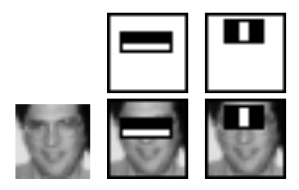
\includegraphics[width=0.45\linewidth]{haar_features2}
  \caption{Primer obeležja za detekciju lica \cite{Viola2001RapidOD}}
  \label{haar_features_img2}
\end{figure}

Oblik obeležja zavisi od namene detektora.
Na slici(\ref{haar_features_img2}) se mogu videti dva tipična obeležja koja su od
interesa za detekciju lica. \\
Prvo obeležje namenjeno je merenju razlike intenziteta osvetljaja regiona čela i očiju.
Ovo obeležje koristi činjenicu da je oblast čela svetlija od očiju. \\
Drugo obeležje poredi intenzitet regiona mosta nosa sa očima, ovde se koristi
činjenica da je region mosta svetliji od očiju. \\

Za dimenziju prozora 24x24 kombinacije svih mogućih varijacija oblika i pozicija
datih obeležja čini skup od oko 160.000 različitih obeležja.
Neki od ovih obeležja neće biti korisni prilikom detekcije željenog objekta.
Veliki broj obeležja će ciljati istu osobinu detektovanog objekta tako da neće
dobrineti povećanoj preciznošću detekcije.
Iz tih razloga moguće je drastično smanjiti i pronaći optimalan broj obeležja
korišćenjem algoritma za mašinsko učenje poput AdaBoost. \\

\subsubsection{AdaBoost}

Kako je već rečeno može se dobiti oko 160.000 obeležja za prozor dimenzije
24x24.
Potrebno je pronaći optimalan broj obeležja za detekciju željenog objekta.
Ukoliko je broj obeležja previše mali detekcija neće biti pouzdana, a ukoliko je
broj obeležja preveliki vreme detekcije je veće. \\
Kako je prikazano na slici(\ref{haar_features_img2}) u primeru detektora lica,
neka obeležja naglašavaju osobine objekta bolje od drugih. \\

Kako bi se odabrao skup korisnih obeležja može se koristiti neki od algoritama
mašinskog učenja. Viola i Jones predlažu modifikovani AdaBoost algoritam. \\

Ideja AdaBoost-a je da se kombinacijom više \emph{weak learner}-a dobija
pouzdana detekcija. \\
\emph{Weak learner} je klasifikator koji ima pouzdanost pogađanja malo bolju
nego nasumično. Odnosno pouzdanost \emph{weak learner}-a mora biti bar malo
iznad 50\%. \\
Kaskadiranjem ovako dobijenih \emph{weak learner}-a može se dobiti \emph{strong
  classifier} \\
Kao rezultat AdaBoost algoritma dobijamo skup optimalnih obeležja, u ovom radu se koristi
model sa skupom od 2913 obeležja.

\subsection{Kaskadni klasifikator}

Osnovni cilj Viola-Jones algoritma je da se na osnovu svih HAAR obeležja u modelu dobije informacija da li se na
trenutnom položaju prozora nalazi traženi objekat (npr. lice).\\
Kako na slici većina skeniranih regiona ne sadrži lice, računanje svih obeležja modela
na svakoj poziciji bi bilo suvišno.
Tako da je korišćenje jednog jakog klasifikatora računski neefikasno. \\

Ukoliko bi se za region koji sigurno ne sadrži lice ranije zaključilo da ga je
moguće odbaciti, dobila bi se značajna ušteda u vremenu detekcije. \\
Organizovanjem obeležja u kaskade i obrazovanjem kaskadnog klasifikatora postiže
se upravo to.
Regioni koji sadrže pozadinu tipično se odbacuju posle jedne ili dve etape
kaskade. \\

\begin{figure}[H]
  \centering
  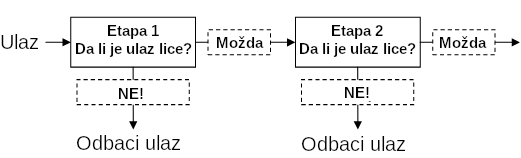
\includegraphics[width=.8\linewidth]{cascade_classifier1}
  \caption{Kaskadni klasifikator \cite{Jensen2008ImplementingTV}}
  \label{cascade_classifier_img1}
\end{figure}

Kako bi se prozori bez lica brzo odbacili predlog je da se jaki klasifikatori
grupišu u etape (eng. \emph{stage}). Ranije etape trebaju da budu dobre u
odlučivanju da li se na posmatranom prozoru definitivno ne nalazi lice.
Ukoliko je to slučaj taj prozor će se brzo odbaciti. \\
Ukoliko rezultat etape ukazuje na to da se na posmatranom prozoru možda nalazi lice, preći
će se na izvršavanje sledeće etape. \\

Konačno ukoliko sve etape u klasifikatoru na analiziranom prozoru daju rezultat
da se na njemu možda nalazi lice može se zaključiti da se na toj poziciji zaista nalazi lice. \\
Zahvaljujući ovome postiže se veoma pouzdan klasifikator sa malim procentnom
pogrešno negativnih (eng. \emph{false negative}) rezultata na krajnjim etapama. \\
Takođe vreme detekcije je značajno skraćeno zbog brzog odbacivanja pozadine
slike. \\

U ovom radu će se koristiti model kaskadnog klasifikatora za
prepoznavanje lica, sa 25 etapa i 2913 obeležja. \\
U prvoj etapi se nalazi samo 9 obeležja, dok taj broj raste do 211 u kasnijim etapama.

\begin{figure}[H]
  \centering
  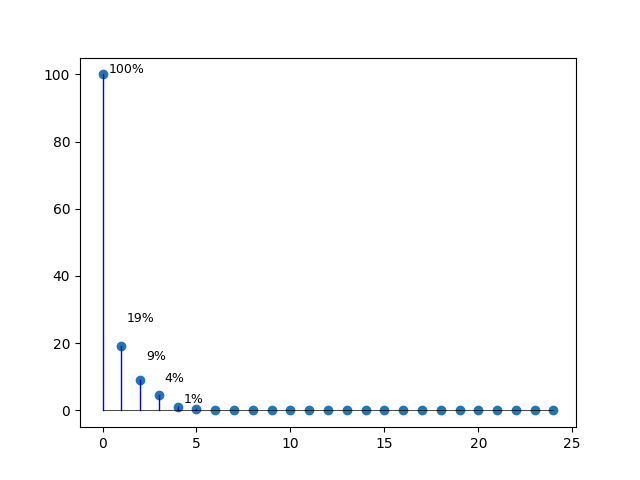
\includegraphics[width=12cm]{cascade_classifier2}
  \caption{Procenat izvršavanja etapa na svim regionima slike}
  \label{cascade_classifier_img2}
\end{figure}

Na slici(\ref{cascade_classifier_img2}) je prikazana statistika izvršavanja
etapa na \emph{Caltech Dataset-u}\cite{CALTECH_DATASET}.\\
\emph{Caltech Dataset} sadrži 450 slika 27 različitih
ljudi pod različitim osvetljenjima, izrazima lica i pozadinama. \\

Vrednosti različitih tačaka na grafu predstavlja procenat izvršavanja date etape
na svih 450 slika. Prva etapa će se naravno uvek izvršiti, dok će se druga etapa
izvršiti samo u 19\% analiziranih prozora, druga 9\% itd... \\
Vidimo da je posle pete etape procenat izvršavanja manji od 1\%. \\

\subsection{Skaliranje slike}\label{image_scaling}

Objekti na slikama mogu biti bliži ili dalji kameri odnosno mogu biti
različitih dimenzija, potrebno je obezbediti da se ona detektuju nezavisno od
veličine. \\

Pošto su obeležja istrenirana da detektuju samo lica koja su iste dimenzije kao
i veličina obeležja potrebno je skalirati sliku ili obeležja kako bi
mogli da se detektuju objekti veći od dimenzija obeležja. \\
Usled toga najmanja dimenzija objekta kojeg je moguće detektovati jednaka je dimenziji obeležja.

\begin{figure}[H]
  \centering
  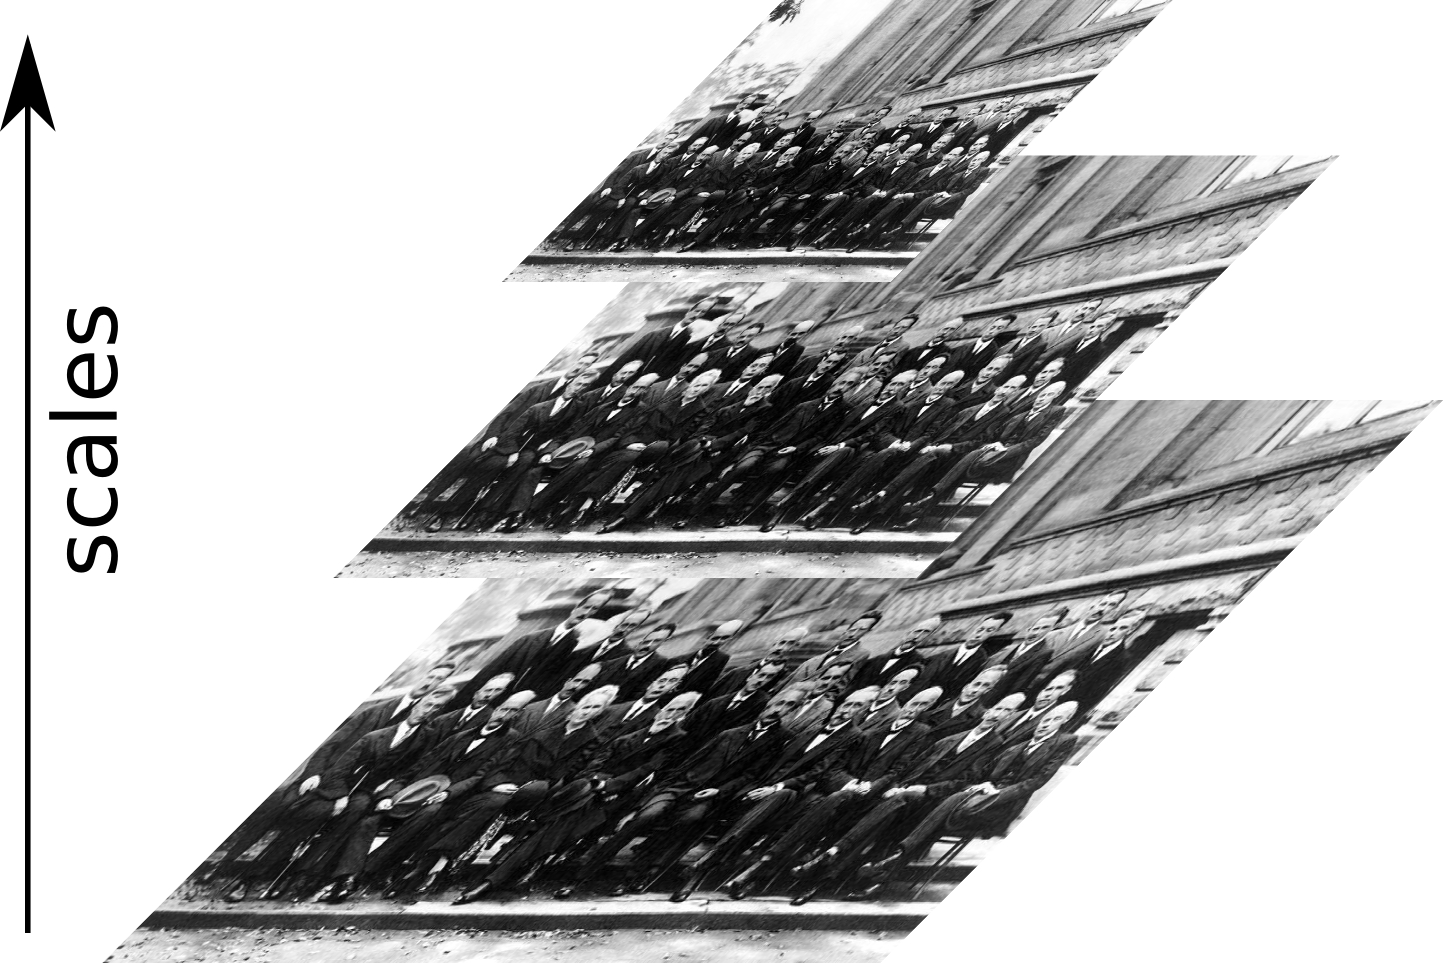
\includegraphics[width=0.45\linewidth]{image_pyramid}
  \caption{Piramida slike\cite{ImagePyramid_web}}
  \label{image_pyramid}
\end{figure}

Ovaj problem je rešen skaliranjem slike.
Na slici(\ref{image_pyramid}) prikazana je piramida skaliranih slika. \\
Detekcija se prvo vrši na slici originalnih dimenzija, nakon toga se dimenzije
slike smanjuju sa nekim faktorom.
Skaliranje se ponavlja sve dok je dimenzija skalirane slike veća od dimenzija
obeležja. \\

Biranjem velikog faktora skaliranja dobija se veća brzina detekcije, ali se može
izgubiti na preciznosti tako što će objekti određenih dimenzija biti ignorisani. \\
Potrebno je naći optimalan odnos brzine i preciznosti. \\

\begin{figure}[H]
  \centering
  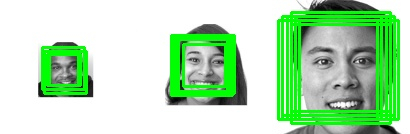
\includegraphics[width=0.8\linewidth]{sixfaces_scaled_res}
  \caption{Različite veličine lica}
  \label{sixfaces_scaled}
\end{figure}

Na slici(\ref{sixfaces_scaled}) može se videti rezultat klasifikatora za 3 lica
različitih dimenzija. \\

\newpage

\subsection{Osetljivost na osvetljaj}\label{lumi_inv_sec}

Objekti se mogu naći pod raznim profilima osvetljenja što uzrokuje značajan problem ovom algoritmu.


\begin{figure}[H]
  \centering
  \parbox{0.4\linewidth}{
    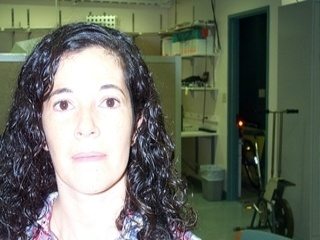
\includegraphics[width=1\linewidth]{overexposed_light}
    \caption{Previše osvetljaja\cite{CALTECH_DATASET}}
    \label{overexposed_light}}
  \qquad
  \begin{minipage}{0.4\linewidth}
    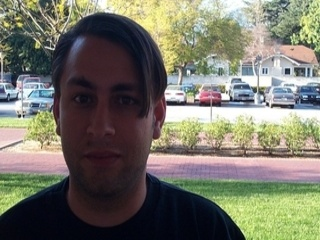
\includegraphics[width=1\linewidth]{underexposed_light}
    \caption{Premalo osvetljaja\cite{CALTECH_DATASET}}
    \label{underexposed_light}
  \end{minipage}
\end{figure}

Na slikama(\ref{overexposed_light}, \ref{underexposed_light}) su prikazana dva
lica koja zbog nepovoljnog osvetljenja nisu detektovane od strane
klasifikatora.
Slika(\ref{overexposed_light}) nije detektovana zbog pristustva prejakog osvetljenja
lica, dok slika(\ref{underexposed_light}) nije detektovana zbog slabog
osvetljenja.  \\

Kao delimično rešenje ovog problema uvedeno je računanje standardne devijacije
prozora koji se detektuje.
Ovo može poboljšati detekciju u nekim slučajevima, ali ne i ekstremnim kao u
prethodnom primeru.

\subsection{Osetljivost na rotaciju objekta}

Dodatna mana ovog algoritma je nemogućnost detektovanja objekata koji su
rotirani. \\
Odnosno moguće je detektovati objekte samo u onom položaju u kojem su prikazani
prilikom treniranja modela. \\
Teoretski moguće je trenirati model za različite uglove rotacije objekta, ali to
bi dodatno povećalo dimenzije modela i smanjilo pouzdanost detekcije. \\

\begin{figure}[H]
  \centering
  \parbox{0.4\linewidth}{
    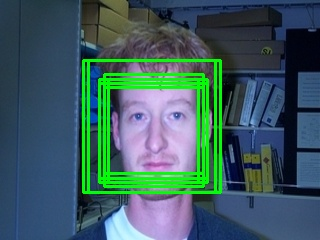
\includegraphics[width=1\linewidth]{rotation_variance}
    \caption{Originalna\cite{CALTECH_DATASET}}
    \label{rotation_variance}}
  \qquad
  \begin{minipage}{0.4\linewidth}
    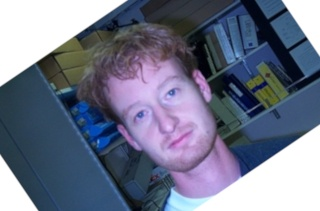
\includegraphics[width=1\linewidth]{rotated_res}
    \caption{Rotirana\cite{CALTECH_DATASET}}
    \label{rotated_res}
  \end{minipage}
\end{figure}